% TikZ plot for operational metrics
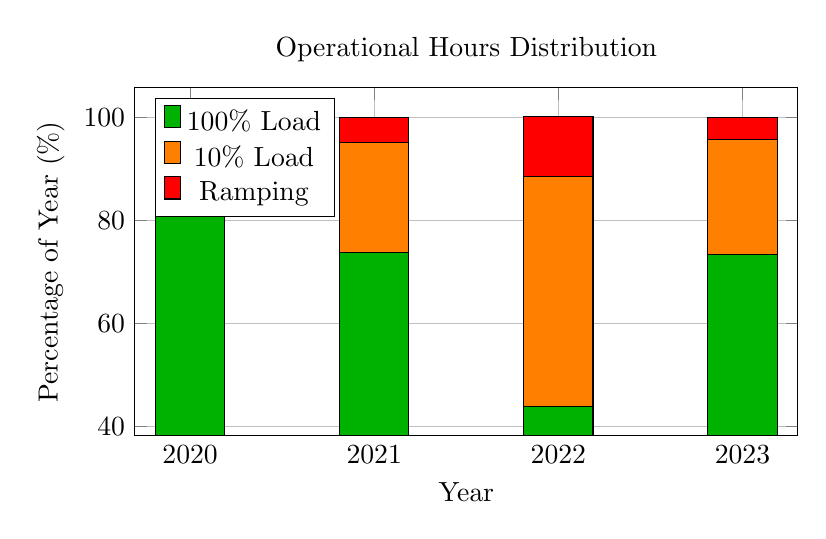
\begin{tikzpicture}
\begin{axis}[
    title={Operational Hours Distribution},
    xlabel={Year},
    ylabel={Percentage of Year (\%)},
    ybar stacked,
    bar width=25pt,
    width=10cm,
    height=6cm,
    xtick=data,
    xticklabels={2020, 2021, 2022, 2023},
    grid=major,
    legend pos=north west,
]

\addplot[fill=green!70!black,draw=black] coordinates {
    (2020, 98.4)
    (2021, 73.7)
    (2022, 43.8)
    (2023, 73.4)
};
\addlegendentry{100\% Load}

\addplot[fill=orange,draw=black] coordinates {
    (2020, 1.1)
    (2021, 21.4)
    (2022, 44.7)
    (2023, 22.3)
};
\addlegendentry{10\% Load}

\addplot[fill=red,draw=black] coordinates {
    (2020, 0.5)
    (2021, 4.8)
    (2022, 11.6)
    (2023, 4.2)
};
\addlegendentry{Ramping}

\end{axis}
\end{tikzpicture}
